\documentclass[11pt]{article}
\usepackage{common}
\usepackage[usenames, dvipsnames]{color}
\usepackage{setspace}
\usepackage{booktabs}
\usepackage{multirow}

\title{CS207 Algorithm Analysis: Kernel Density Estimation}
\author{Gioia Domined\`o \and Nicolas Drizard \and Kendrick Lo \and Malcolm Mason Rodriguez}

\begin{document}
\maketitle{}

\pagestyle{plain}
\pagenumbering{arabic}

\section{Introduction}

Kernel Density Estimation (KDE) is a non-parametrical statistical technique that is used to estimate the probability density function (PDF) of a random variable based on a finite data sample\footnote{https://en.wikipedia.org/wiki/Kernel\_density\_estimation}.  Mathematically, we can denote the KDE of the PDF of independent and identically distributed (\textit{iid}) random variables $X=\{x_1, x_2, ..., x_n\}$ as:

\begin{equation} \label{eq:kde}
\hat{f}_h(x) = \frac{1}{n} \sum_{i=1}^n K_h(x - x_i) = \frac{1}{nh} \sum_{i=1}^n K \Big( \frac{x - x_i}{h} \Big)
\end{equation}

\noindent where $K(\cdot)$ represents the \textit{kernel} and $h$ represents the \textit{bandwidth} (i.e. a smoothing parameter). We note that $\hat{f}_h(x)$ denotes the estimated PDF at a particular point $x$, and that the entire data set $X$ is used to calculate it. \medskip

\noindent Various kernels are used in practice (e.g. Gaussian, Epanechnikov, exponential, etc.), all of which meet the criteria of being non-negative functions with mean zero that integrate to one. Similarly, different (strictly positive) values of $h$ can be chosen depending on the data set in question. Figure \ref{fig:kde_params} illustrates how the choice of these two parameters affects the shape of the estimated PDF.

\begin{figure}[h!]
\centering
\subfloat[Changing the kernel (bandwidth$=0.2$)]{\label{fig:kde_params_k}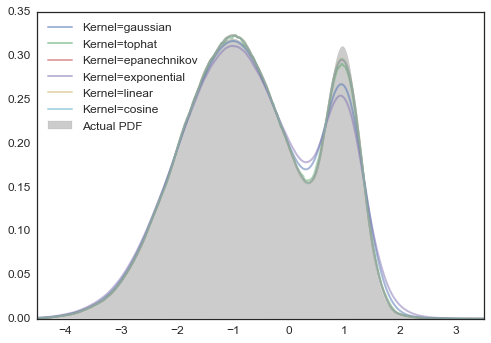
\includegraphics[width=3in]{img/change_k}}
\subfloat[Changing the bandwidth (gaussian kernel)]{\label{fig:kde_params_bw}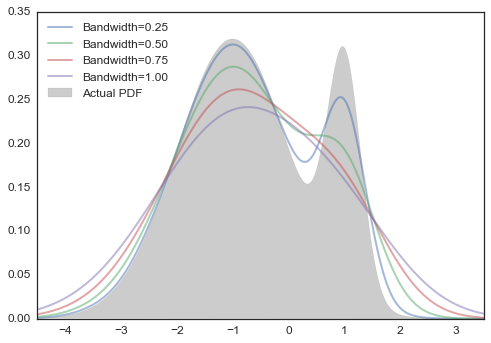
\includegraphics[width=3in]{img/change_bw}}
\caption{Impact of KDE parameters}
\label{fig:kde_params}
\end{figure}

\newpage

\section{Algorithm}

For ease of comparability, we used a consistent set of parameters for all our experiments: a Gaussian kernel and a bandwidth of $0.2$. Figure \ref{fig:sample_kde} shows the result of running the algorithm with these parameters on 100K one-dimensional random variables drawn from a bimodal distribution, where the PDF is plotted at 1K evenly-spaced points.

\begin{figure}[h!]
\centering
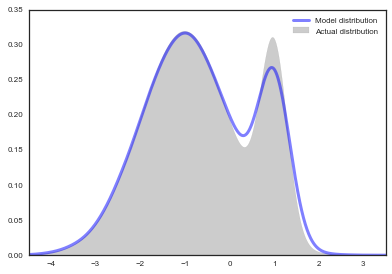
\includegraphics[width=4in]{img/sample_kde.png}
\caption{Sample KDE output}
\label{fig:sample_kde}
\end{figure}

\noindent We started by implementing a ``pure" Python version of KDE; in keeping with that objective, we only used lists. We can see from the code below that the KDE algorithm is a direct application of Equation \ref{eq:kde}. The double loop, which is necessary due to the use of lists, immediately stands out as a significant source of inefficiencies.

\begin{singlespacing}
\begin{scriptsize}
\begin{verbatim}
def naive_kde(x, x_grid, h):
    '''
    Calcalates the KDE PDF estimate, based on a Gaussian kernel.
    Inputs
    ----------
    x      : A list of iid random variables that are used to calculate the KDE estimate
    x_grid : A list of values along which to calculate the KDE estimate
    h      : Float, the bandwidth parameter for the KDE estimate
    Returns
    ----------
    A list of KDE estimates for all values of x_grid.
    '''
    global N # number of iid random variables
    estimates = [0] * len(x_grid)
    
    for j, gridpt in enumerate(x_grid):
        for i in range(N):
            val_in_sum = gaussian((x[i] - gridpt) / h)
            estimates[j] += val_in_sum
        
        estimates[j] = estimates[j] / (N * h)
    
    return estimates
\end{verbatim}
\end{scriptsize}
\end{singlespacing}

\newpage

\noindent Before moving on to the Scikit Learn implementation, we tested the effect of switching from lists to Numpy arrays and vectorizing the inner loop. This simple change, which is shown in the code below, reduced the runtime from nearly 300 seconds to just over 1 second!

\begin{singlespacing}
\begin{scriptsize}
\begin{verbatim}
def vectorized_kde(x, x_grid, h):
    '''
    Calcalates the KDE PDF estimate, based on a Gaussian kernel.
    Inputs
    ----------
    x      : An array of iid random variables that are used to calculate the KDE estimate
    x_grid : An array of values along which to calculate the KDE estimate
    h      : Float, the bandwidth parameter for the KDE estimate
    Returns
    ----------
    An array of KDE estimates for all values of x_grid.
    '''    
    global N # number of iid random variables

    estimates = np.zeros(len(x_grid))
    
    for j, gridpt in enumerate(x_grid):
        val_in_sum = gaussian((x - gridpt)/h)  # returns vector of dim N
        estimates[j] = np.sum(val_in_sum) / (N * h)
    
    return estimates
\end{verbatim}
\end{scriptsize}
\end{singlespacing}

\section{ScikitLearn Optimizations}



\begin{table}[h!]
\centering
\begin{tabular}{@{}ll@{}}
\toprule
Implementation			& Runtime (seconds)       	\\
\midrule
Naive Python			& 298.28				\\
Vectorized Python		& 1.34				\\
Scikit Learn			& 5.73				\\
\bottomrule
\end{tabular}
\caption{Comparing one-dimensional KDE implementations}
\label{compare_kde}
\end{table}


%\section{Numpy Implementation}
%
%\section{ScikitLearn Implementation}

%5-6 pages max, please
%one per group!
%choose an algorithm, from someplace like sklearn, which has an optimization. By optimization I mean code written in C and integrated, or code written in cython or SWIG or similar (optionally you could choose a more algorithmic kind of optimization, but this is not explicitly encouraged since this is a computer science and not numerical programming class)
%explain why, in your opinion, the writers felt the need of an optimization
%to do this, explain the basic algorithm by writing an implementation in pure python. You can use the project's test examples to make sure your implementation is correct.
%explain the logic of the optimization

%Hey? I?ve looked over the scikit learn functions, and for the paper I would propose doing  Kernel Density Estimation. In sklearn, they use trees and Cython to speed things up, and the .pyx file is there? so it should not be too onerous to make up, I mean, write something based on that. Also, the author of the code wrote a blog article and we can draw further observations from those:  e.g. http://jakevdp.github.io/blog/2013/12/01/kernel-density-estimation/

\end{document}
